\chapter{Detecting Abnormalities in Materials Data}  \label{chap:pyqalloy}


\section{Introduction} \label{pyqalloy:sec:intro}

As explored in Chapter~\ref{chap:ultera}, handling of the "real" materials data requires many complex steps that introduce many potential points of failure, prompting investigations into the quality of the resulting datasets and the provenance of errors once they are identified. The first component of such efforts includes \emph{validity} of the data, which can generally be accomplished based on conformance to some defined specification and implemented in the data pipelines, like the ones discussed earlier in Section~\ref{ultera:sec:pipeline} or solutions built around frameworks like \texttt{pydantic} \cite{WelcomePydantic}.

Validating the data, however, does not, per se, make it correct, and most of the errors known to be common in alloy datasets, in fact, cannot be caught. Furthermore, even secondary hand-checking of the data, often taken as ground truth in parsing efforts, can often be very flawed since data may appear perfectly valid at a glance or be incorrectly interpreted.

This necessitates an alternative approach to ensuring high quality based around detection of abnormalities in the validated datasets, followed by re-verification of the suspicious data. In ULTERA Database, this has been implemented through \texttt{PyQAlloy} software, or \textit{Python toolset for Quality of Alloy data}, which connects to it and deploys several methods custom-designed for compositionally complex materials (CCMs) or high entropy alloys (HEAs) data, as shown schematically in Figure~\ref{pyqalloy:fig:schematic} and discussed throughout Section~\ref{pyqalloy:sec:abnormalities}.

\begin{figure}[H]
    \centering
    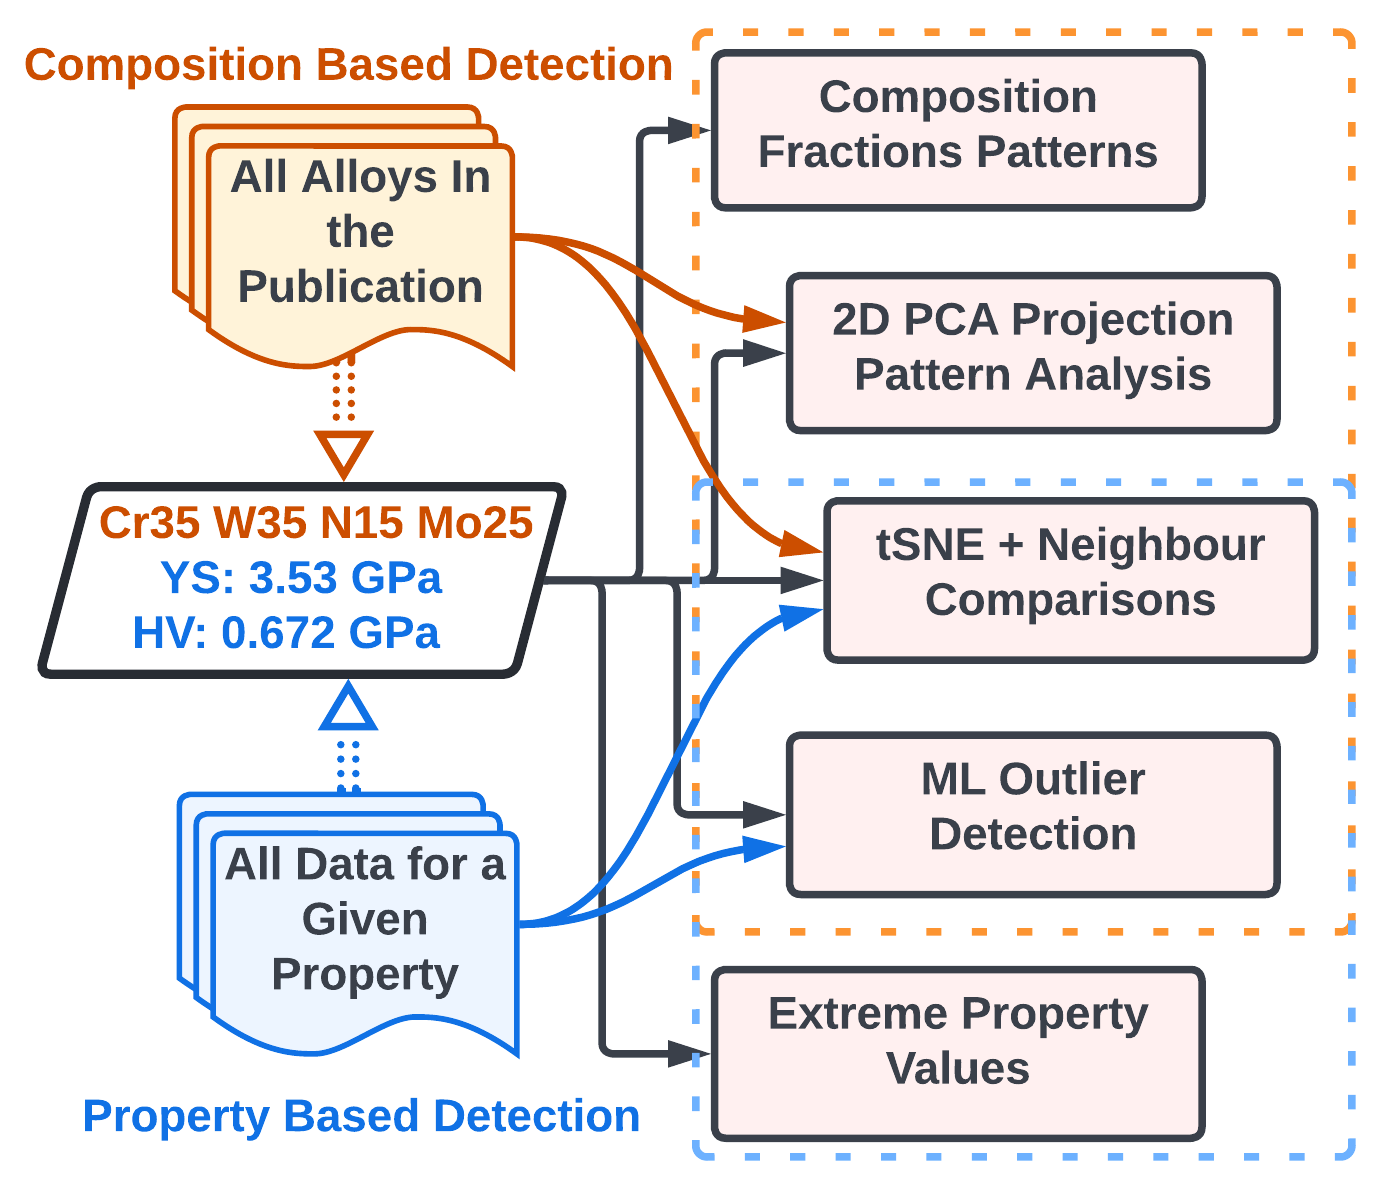
\includegraphics[width=0.6\textwidth]{pyqalloy/AbnormalCompositionDetection_v1.png}
    \caption{Schematic of \texttt{PyQAlloy} software operating in several contexts to detect and investigate common abnormalities discussed in Subsections \ref{pyqalloy:ssec:extreme} through \ref{pyqalloy:ssec:global}.}
    \label{pyqalloy:fig:schematic}
\end{figure}

Internally, \texttt{PyQAlloy} leverages several contexts each data exists in, ranging from a single aspect of it, through individual composition-structure-property relations, to the entire ULTERA database. Thanks to such a multi-context approach, a wide variety of errors can be caught.

\section{Common Abnormalities and Detection of Errors} \label{pyqalloy:sec:abnormalities}

Most commonly, the errors present in properly validated alloy datasets have to do with misreported compositions, numerical values, or both, which can add noise to the dataset or systematically skew it. The latter is particularly problematic to machine learning (ML) studies, as it can very significantly alter the extrapolation ability of the model. Throughout this Section, several common abnormalities are discussed alongside examples of errors that can cause them, starting from the least complex ones.

\subsection{Extreme Values} \label{pyqalloy:ssec:extreme}

The simplest abnormality one can detect, both in terms of concept and implementation, has to do with abnormally high or low values being present, which can be readily monitored through histograms, such as the one shown for old ULTERA hardness data in Figure~\ref{pyqalloy:fig:extreme}, constructed for each individual numerical value encountered in the database. Within ULTERA, such histograms are maintained alongside more descriptive extreme data tables and updated daily to inform responsible team members of possible errors.

\begin{figure}[H]
    \centering
    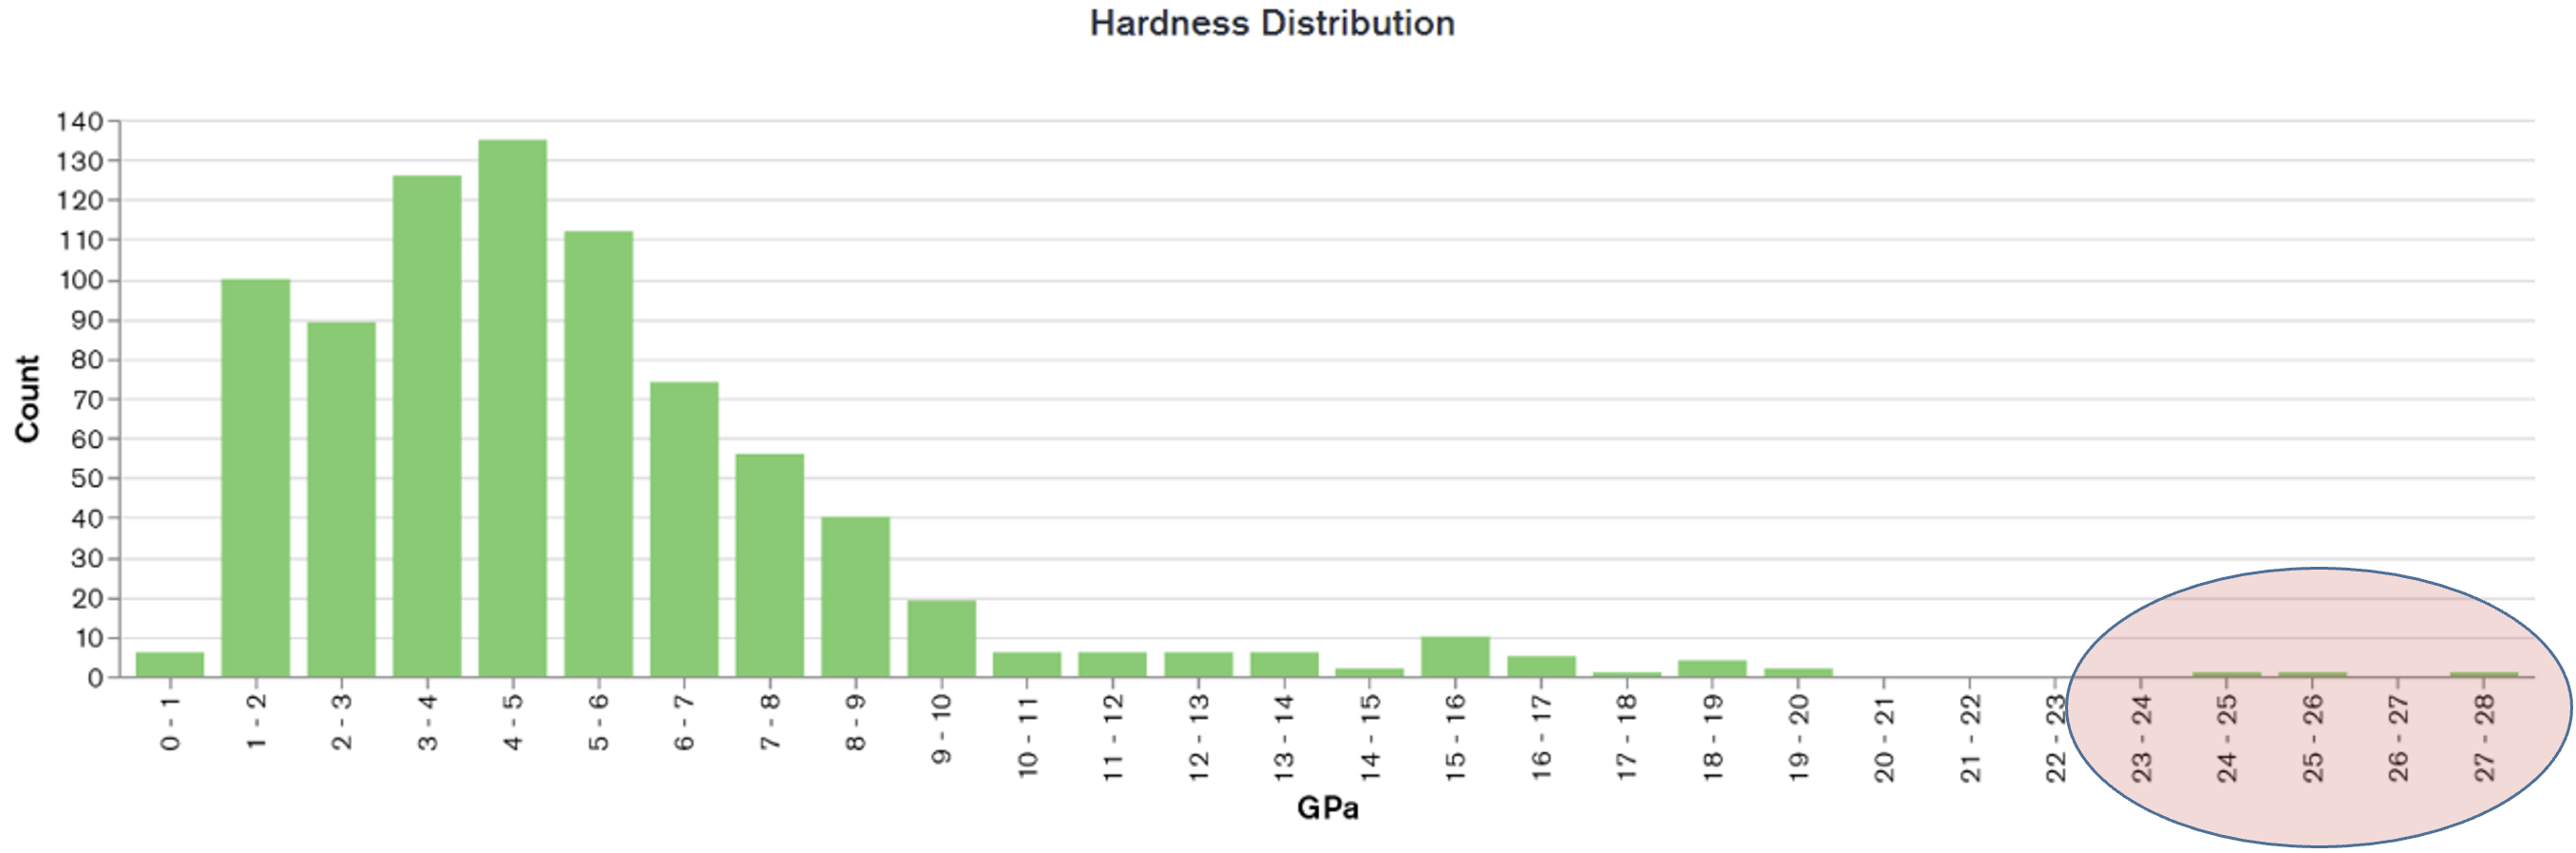
\includegraphics[width=0.95\textwidth]{pyqalloy/pyqalloy_extremevalues.png}
    \caption{A legacy, pre-curation ULTERA hardness data histogram. The extreme, out-of-distribution values (highlighted) indicate possible misinterpretation. Two out of three were misreported due to the "extra 0" typo, while the highest one (27.5 GPa) was properly reported \ch{Mo_{40.5}Ni_{40.5}B_{10}Si_9} extremely hard metallic glass \cite{Kim2016DevelopmentRatios}. A similar analysis applies to extremely low values.}
    \label{pyqalloy:fig:extreme}
\end{figure}

More elaborate extreme value detection tools can also analyze the values in the context of expectations of what should be contained in the database. For instance, since the ULTERA database is focused on \emph{high} entropy alloys, \emph{low} entropy multi-component alloys, like the ones shown in Figure~\ref{pyqalloy:fig:lowentropy}, may be considered extreme in this context. This exact approach has been successfully used in ULTERA to fix several data points for which a fraction of one of the components has been accidentally inflated, causing the alloy to have a single principal element.

\begin{figure}[H]
    \centering
    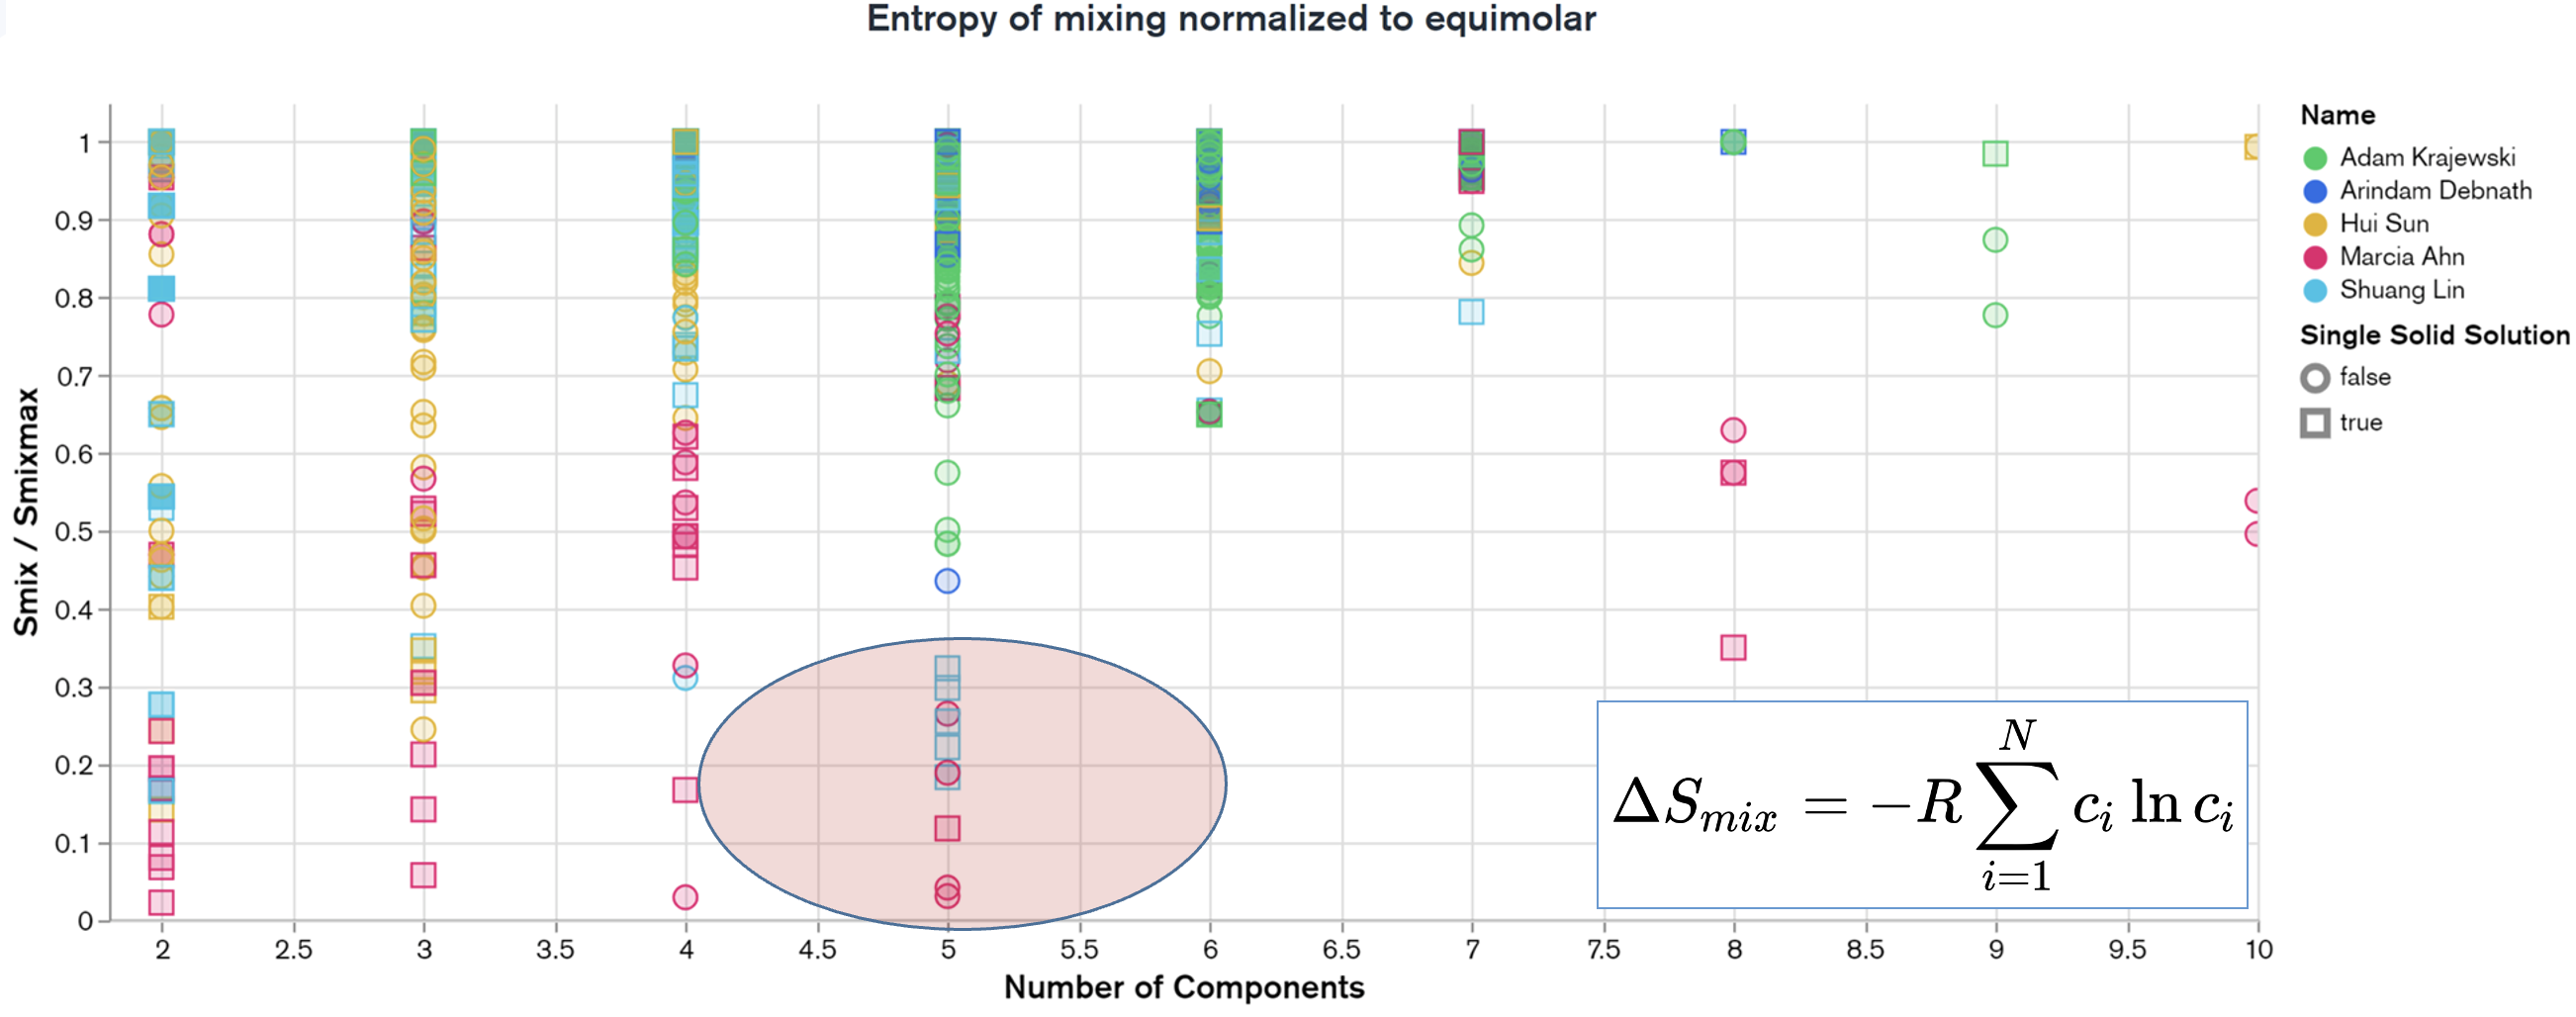
\includegraphics[width=0.95\textwidth]{pyqalloy/pyqalloy_entropy.png}
    \caption{An example of extreme value detection in secondary data characteristics relative to expectations. The legacy, pre-curation ULTERA data plot of the ideal mixing entropy of a given alloy divided by the maximum ideal mixing entropy corresponding to the number of components present (value of $1$ indicates equimolar alloy). Extremely low values in this metric indicate a high likelihood of "double click" or "missing comma" typos at data parsing, which resulted in one element becoming highly dominant.}
    \label{pyqalloy:fig:lowentropy}
\end{figure}


\subsection{Single Composition Patterns} \label{pyqalloy:ssec:singlecomp}

Similar to detecting abnormalities in the individual numerical values, one can also, relatively simply, detect specific abnormalities in the individual reported compositions. The most obvious yet the most common abnormality pattern deals with sums of atomic fractions being both (1) around $100$ or $1$ (within, e.g., $10$ or $20\%$ of them), and (2) not precisely $100$ or $1$, with minor deviations (e.g., $0.2\%$) allowed to account for numerical precision.

For instance, in the published (unprocessed) version of one of the literature datasets mentioned in Section~\ref{ultera:sec:datadescription} one can find a number of alloys reported from study by \citet{Stepanov2019EffectContent}, including \texttt{Cr20 Mn25 Fe40 Ni15 Al14}, which look fine at first but sum to $114$ what gets immediately detected by \texttt{PyQAlloy}'s \texttt{SingleCompositionAnalyzer} class. In this case, the researcher parsing the publication consistently forgot to subtract a fraction of added Al from the base alloy, causing the error to appear in 12 data points systematically and causing models to overestimate the strengthening effect of Al reported for these alloys \cite{Stepanov2019EffectContent}.

Another example, with a different root cause, has to do with 9 data points extracted from a well-known study by \citet{Lu2017DirectlyRange}, which included compositions like \texttt{Cr16 Fe16 Co16 Ni34.4 Al16} summing to $98.4$. In this case, the underlying cause for the error was likely incorrect normalization of the formula to sum to $100$, which in most circumstances could be considered noise, but in this study, it introduced significant error as the study investigated a narrow compositional range around a eutectic point; thus the errors became on the order of the study's domain and skewed the interpretation dramatically.


\subsection{Single Study Patterns}   \label{pyqalloy:ssec:singlestudy}

Going beyond individual values, one can leverage the fact that individual studies typically follow a limited number of approaches when it comes to setting up a hypothesis to be verified. The three that cover the vast majority of high entropy alloy studies are (1) gradually modifying an alloy in one or more ways, like adding a new element or mixing it with another alloy, (2) combinations or permutations of elements following particular pattern, like equimolar (equal fractions) or quantized (e.g., all fractions are $20\%$ multiples) alloy screenings \cite{Elder2023ComputationalDown-selection, Elder2023ComputationalValidation}, or (3) are actively driven and follow no pattern at all \cite{Rao2022MachineDiscovery}. 

When linearly projected to some lower-dimensional space of choice, using, for instance, principle component analysis (PCA), the resulting patterns fall into two categories. The first case typically follows one or more linear patterns with uniform distance between points (not required, per se), as linear trends in the high dimensional space can be preserved. Meanwhile, the second and third cases will typically result in a largely disordered pattern (given enough components) as there is no underlying low-dimensional pattern based on which the high-dimensional elemental space is being populated. Figure~\ref{pyqalloy:fig:expectedpatterns} depicts examples of both of these expected patterns.

\begin{figure}[H]
    \centering
    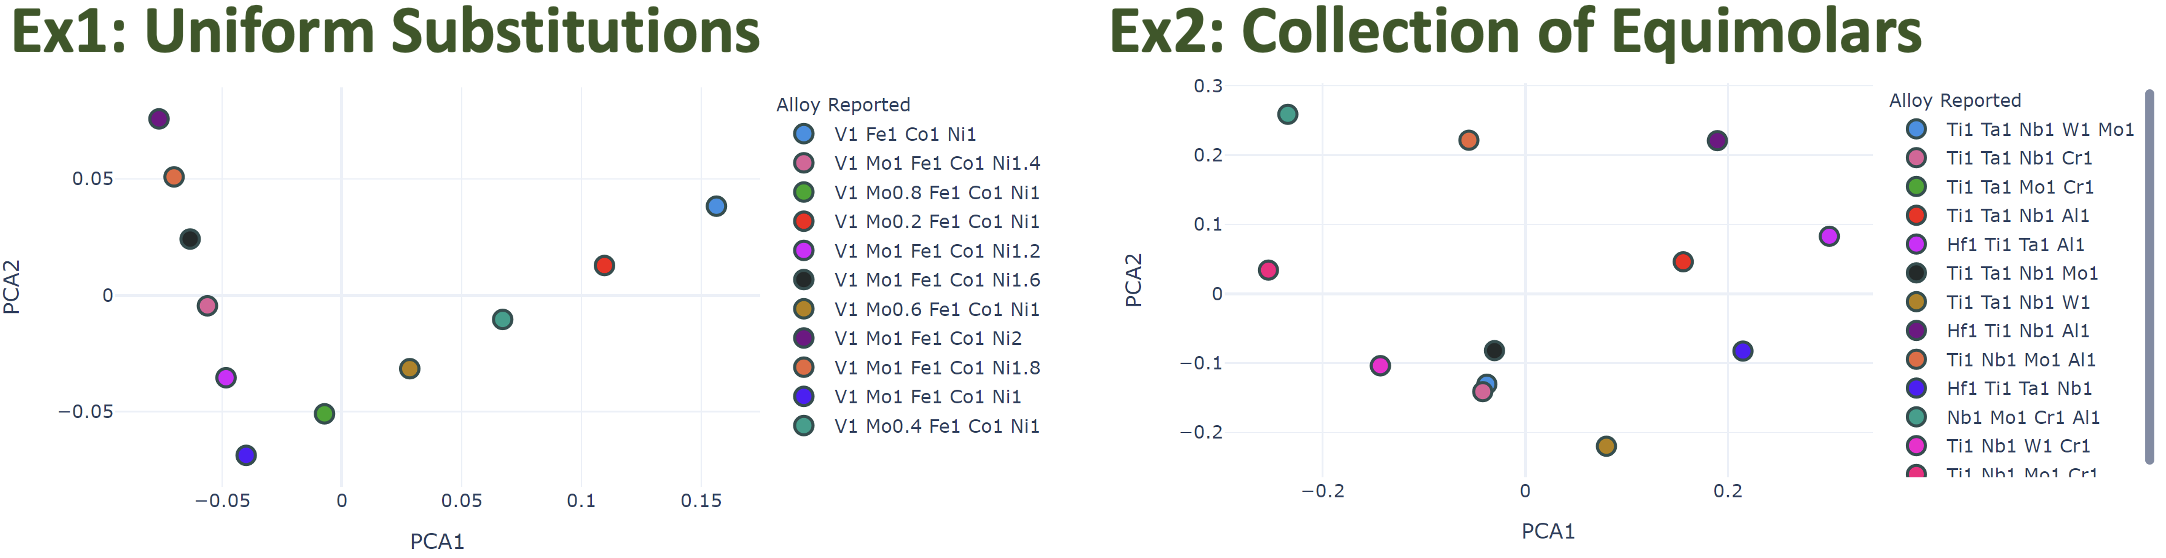
\includegraphics[width=0.95\textwidth]{pyqalloy/pyqalloy_ExpectedPCAPatterns.png}
    \caption{Expected patterns in the PCA projections of high entropy alloy composition vectors onto a 2D plane common for the vast majority of alloy design studies, which either (left) take an alloy and progressively modify it through elemental substitutions or mixing with another alloy in one or more ways, resulting in one or more linear patterns, or (right) test many different elemental combinations that are thought to possibly work well in the application in an anti-systematic fashion (in chemical space) does not follow any lower dimensional pattern and results in a point cloud. Breaks in these patterns, like out-of-line points or anisotropic point clouds, indicate possible errors and should be screened.}
    \label{pyqalloy:fig:expectedpatterns}
\end{figure}

While the second case of disordered embedding patterns cannot be easily exploited for abnormality detection, the breaks in single or multiple linear patterns can be taken advantage of in a semi-automated way through \texttt{PyQAlloy}'s \texttt{SingleDOIAnalyzer} class.

For instance, in an older version of the ULTERA dataset, a set of alloys from the study by \citet{Wang2009AtomicAlloy}, included \texttt{Ti0.5 Cr1 Fe1 Co1 Ni1 Cu0.5 Al0.25}, which appeared correct on its own, but when put in the context of other alloys from the study it broke the expected linear pattern. It was caught by \texttt{PyQAlloy} and then found to be \texttt{Ti0.5 Cr1 Fe1 Co1 Ni1 Al1} in the publication; as depicted in Figure~\ref{pyqalloy:fig:patternbreak1}.


\begin{figure}[H]
    \centering
    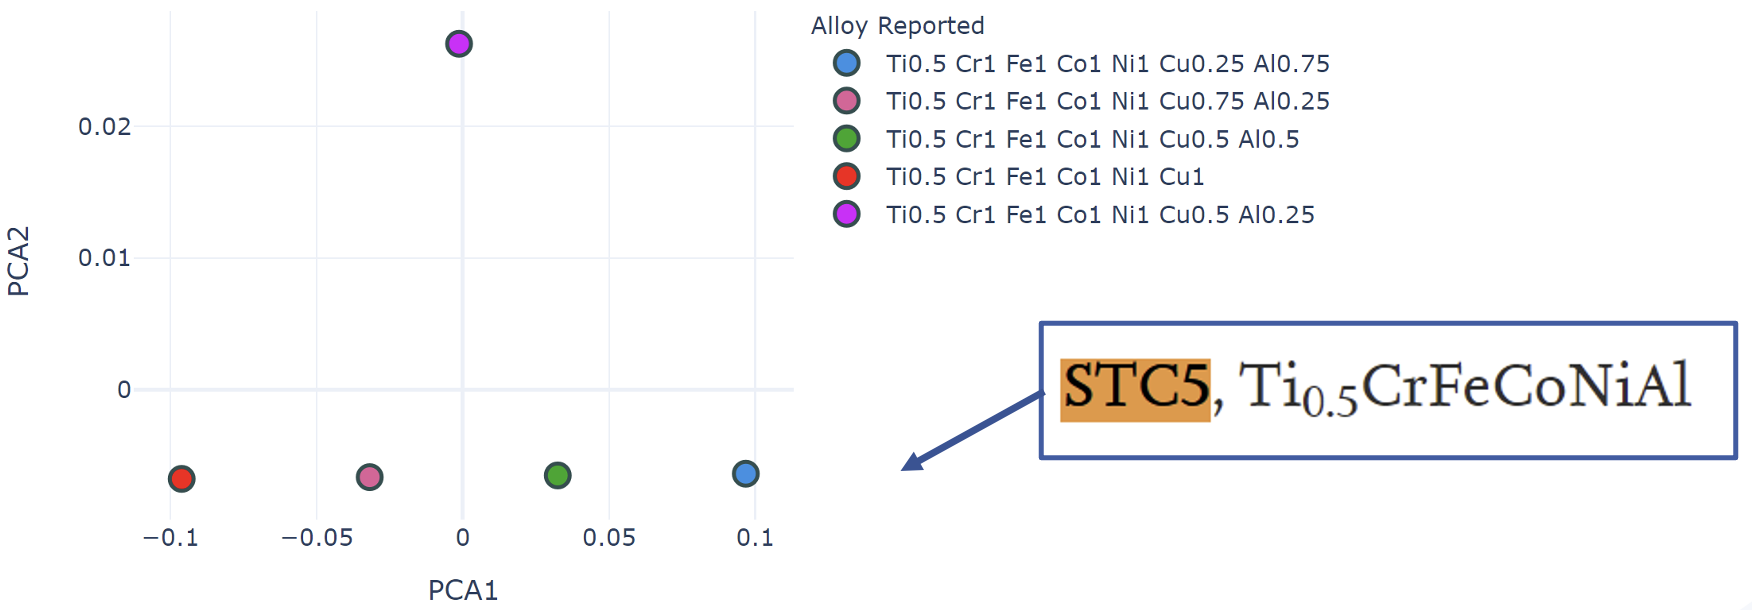
\includegraphics[width=0.95\textwidth]{pyqalloy/pyqalloy_HumanError.png}
    \caption{An example of an out-of-line pattern was detected in a literature review study. It was caused by the researcher parsing a publication incorrectly, noting the composition relative to the source \cite{Wang2009AtomicAlloy}. Composition similar to other points makes it look right; thus, such errors are nearly impossible to catch using other methods.}
    \label{pyqalloy:fig:patternbreak1}
\end{figure}


In addition to typing or copying errors, such single study pattern analysis can also highlight interpretation errors, as such cases tend to break every time a fraction of some component goes to $0$. For instance, in an older version of the ULTERA dataset, a set of 4 alloys from a study by \citet{Amigo2019MechanicalApplications} was reported after passing validations. However, when processed through \texttt{PyQAlloy}, it was found that one of the alloys, with no \texttt{Fe} reported, broke the pattern as the fraction of \texttt{Ta} was expected to drop to $0$ instead, as illustrated in Figure~\ref{pyqalloy:fig:patternbreak2}. Further verification revealed that all 4 have been misreported, as the original study used composition notation which (a) reported atomic fractions as prefixes rather than suffixes of the element symbol, (b) assumed Ti to have the "balance" fraction of $100$ less the sum of other elements, and (c) used weight fractions, which collectively broke the pattern.


\begin{figure}[H]
    \centering
    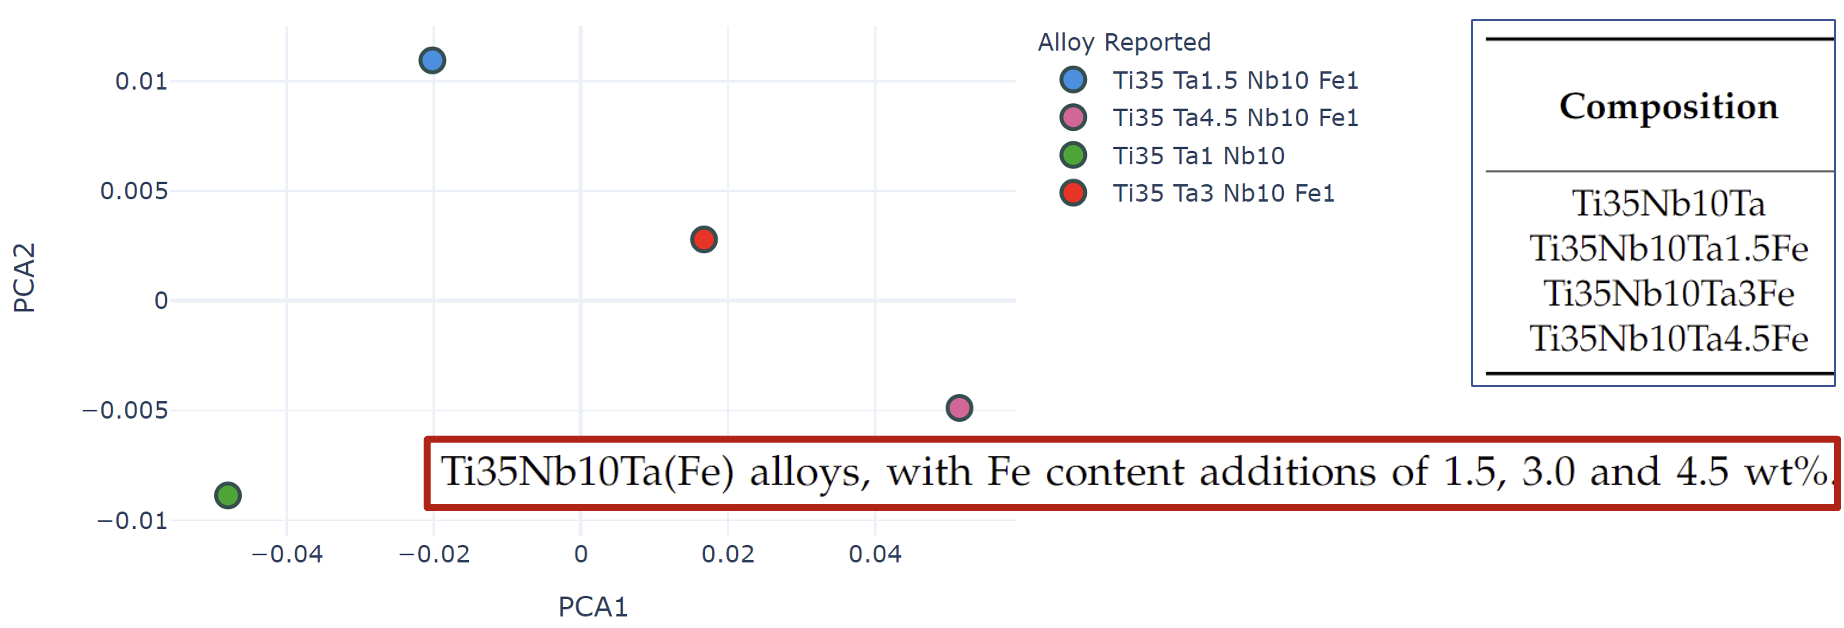
\includegraphics[width=0.95\textwidth]{pyqalloy/pyqalloy_CompositionNotation.png}
    \caption{An example of an out-of-line pattern detected in a literature review study, in which chemical formulas present in the source publication \cite{Amigo2019MechanicalApplications} are correctly parsed. However, they are shorthand composition notations rather than actual chemical formulas of the studied material and must be interpreted; thus, they are incorrectly reported. Such misinterpretations typically follow some incorrect patterns locally but fail to do so if any component is removed or added to the mix, as depicted here.}
    \label{pyqalloy:fig:patternbreak2}
\end{figure}


\subsection{Global Patterns} \label{pyqalloy:ssec:global}

Lastly, one can also leverage the collected ULTERA Database to detect abnormalities between different studies, which can be a powerful technique, especially in cases where they report few data points individually. For instance, a single alloy of \texttt{Hf3 Mo1 B14 Si10} has been previously reported from a study by \citet{Yu2012TensileTemperatures} and did not appear suspicious, except to a person possessing expert knowledge. However, when \emph{entire database} was passed through \texttt{PyQAlloy}'s \texttt{AllDataAnalyzer} class, it was found to be in the neighborhood of other Hf-Mo-B-Si alloys reported in other works based on its t-distributed stochastic neighbor embedding (t-SNE) \cite{HintonStochasticEmbedding}, but at the same time be very far from any other member of this neighborhood based on the DBSCAN clustering \cite{Ester1996ANoise}, as depicted in Figure~\ref{pyqalloy:fig:patternglobal}. After verification, it was found that the fraction of Mo ($73\%$) has been missing.

\begin{figure}[H]
    \centering
    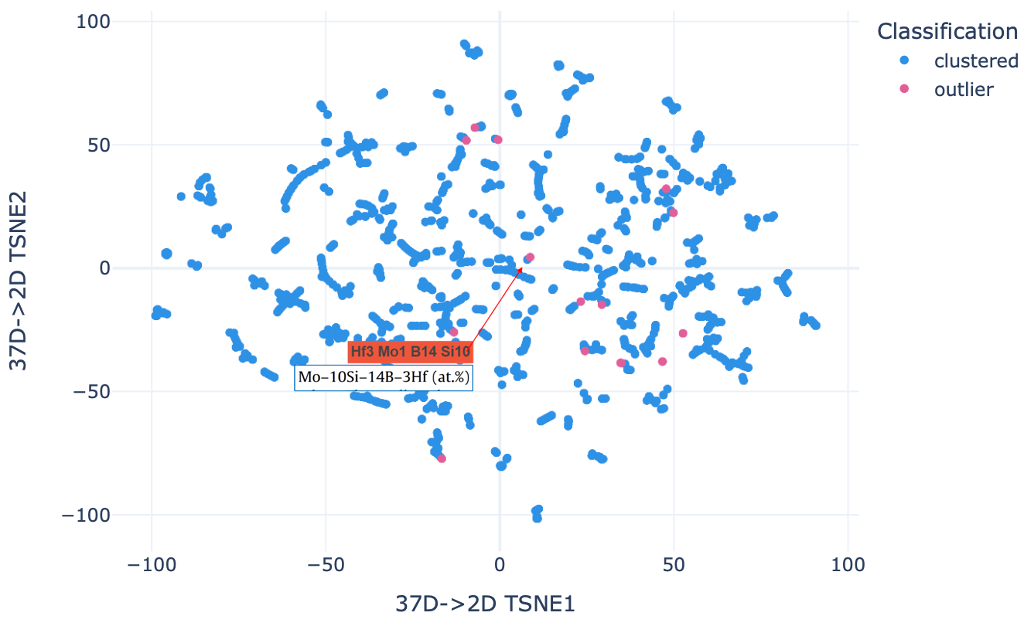
\includegraphics[width=0.95\textwidth]{pyqalloy/PyQAlloy_tSNE+DBSCAN.png}
    \caption{2D tSNE embedding of all chemical compositions present in ULTERA based on alloy neighborhoods overlaid with outliers detected through the DBSCAN method operating in the high-dimensional real composition space. Singular outliers between tSNE clusters are expected and indicate novel compositions, while outliers within clusters indicate far-removed members of an alloy family, which are likely incorrect. The highlighted \ch{B-Hf-Mo-Si} alloy is close to other alloys in that system, but a fraction of \ch{Mo} was omitted by the parsing researcher. In the depicted case, lower-level methods did not detect abnormality because only one alloy was reported.}
    \label{pyqalloy:fig:patternglobal}
\end{figure}

\section{Software Implementation} \label{pyqalloy:sec:software}

The majority of the abnormality detection methods developed for ULTERA have been implemented as a user-tool \texttt{PyQAlloy}, which was released as a free, open-source software (FOSS) under the MIT license. It is available (1) as source code through a GitHub repository at \href{https://github.com/PhasesResearchLab/PyQAlloy}{github.com/PhasesResearchLab/PyQAlloy}, (2) through the PyPI, and (3) through the \texttt{conda-forge} channel. It is automatically tested across several platforms on a periodic basis. Furthermore, its documentation and use examples were made available through \href{https://pyqalloy.ultera.org/}{pyqalloy.ultera.org} web page.




\printbibliography[heading=subbibintoc]